\chapter{HCCP: Heterogeneous Clustering and Control Protocol}
\label{ch:HCCP_intro}

HCCP 
is a method for describing and advertising  the internal resources of wireless 
sensor motes, and using the strengths of the motes to increase message throughput
or extend the lifespan of 
the network. Once motes are aware of their internal resources, they should 
choose clusterheads based on the resources available. For 
example, motes that are assigned the clusterhead role use more energy. 
Therefore, motes that have extra batteries should be chosen as a clusterhead 
before motes without extra batteries. 

\begin{figure}[t]
	\centering
		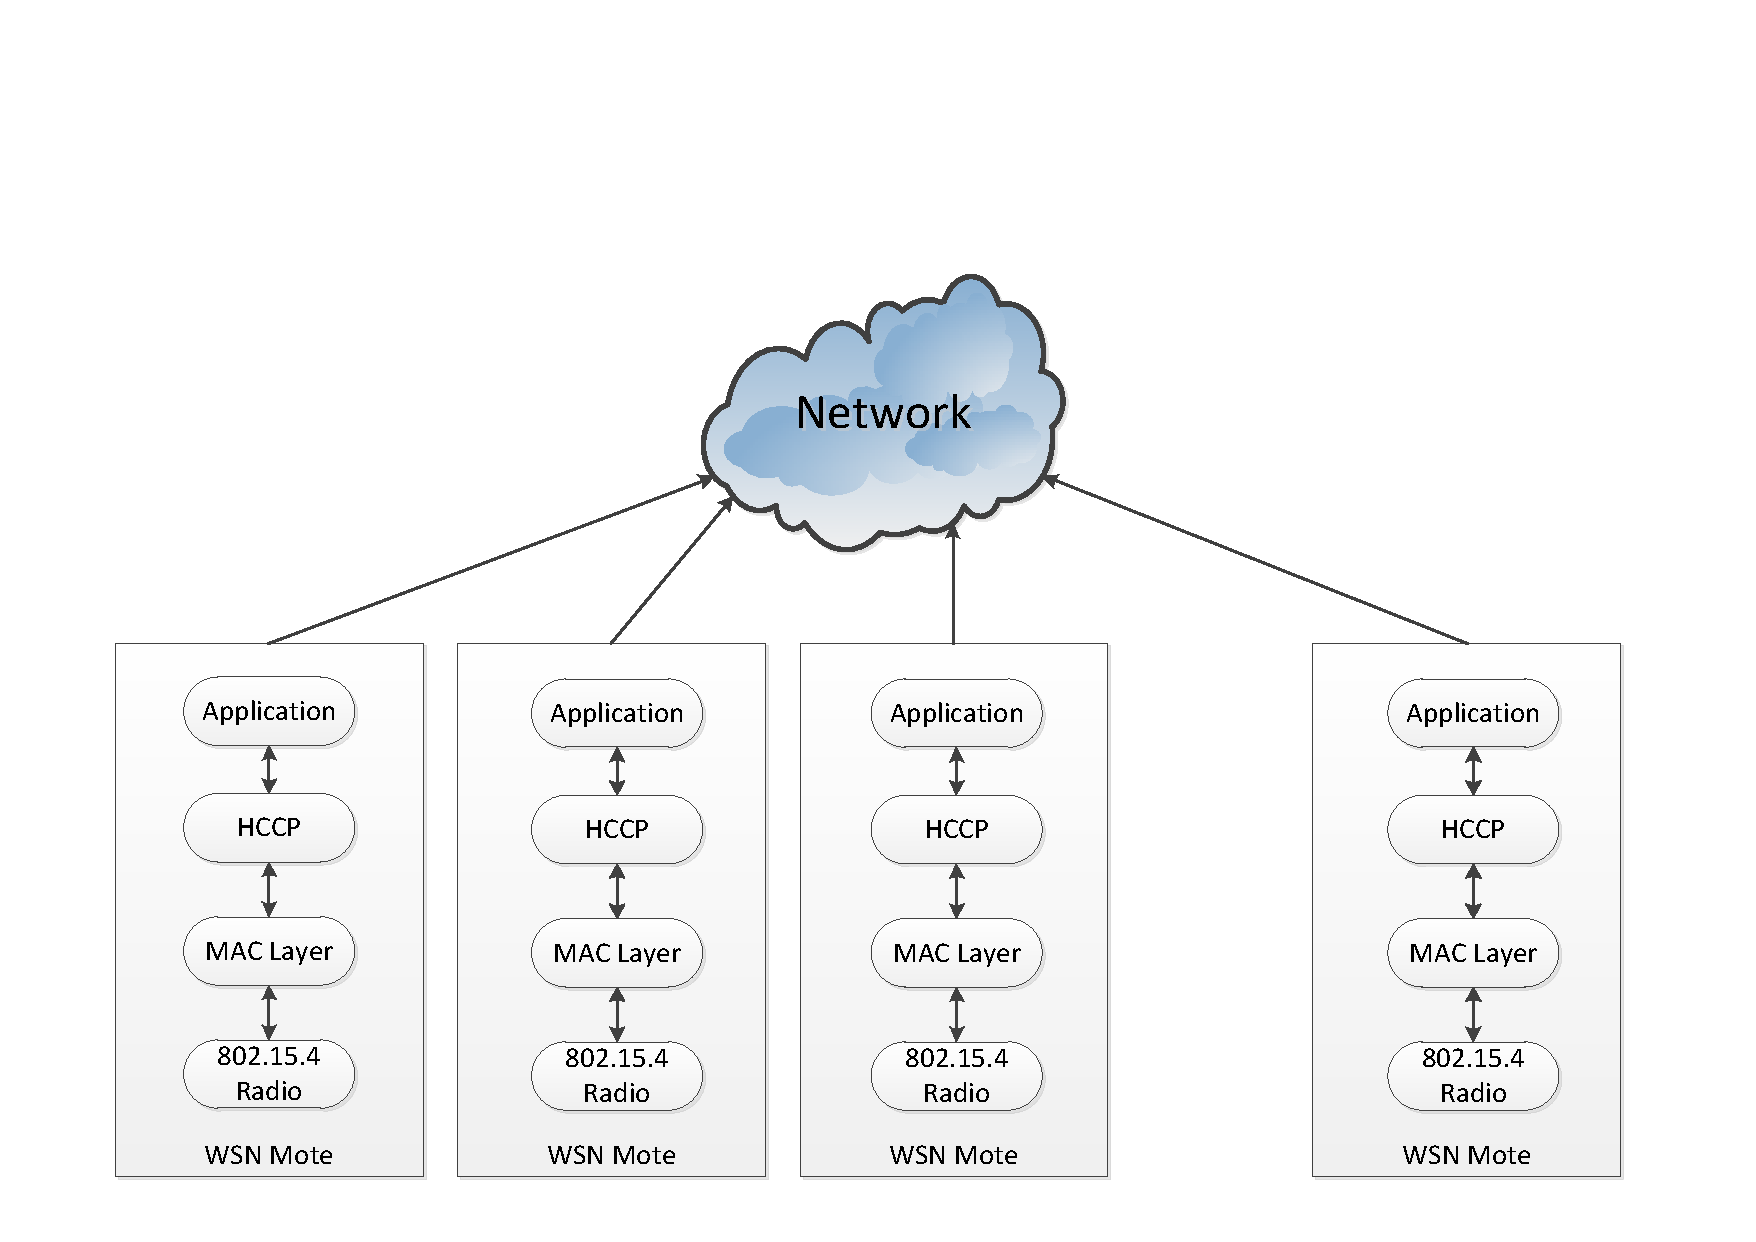
\includegraphics[width=\textwidth]{images/protocol/HCCPAsMiddleWare.pdf}
	\caption{HCCP uses existing MAC protocols and can be used by any application, acting as middleware.}
	\label{fig:images_protocol_HCCPAsMiddleWare}
\end{figure}

A mote should not only be aware of its resources, but it should also be aware 
of the requirements of the network. This is a consideration because the topology 
of WSNs are prone to change due to the battery-powered nature of its 
components (e.g., a mote with a dead battery will change the topology of the 
WSN).  Also, motes may move in the network (by some external force such as a 
person moving the mote), further changing the topology of the network.  To 
handle this unpredictability, the motes need to be aware of the motes nearby, 
but not waste excessive energy discovering them.  

HCCP acts as middleware between the MAC layer and the application layer of the 
mote, as shown in Figure~\ref{fig:images_protocol_HCCPAsMiddleWare}. 
The application layer queues messages that are ready to send, HCCP takes the
messages and sends them to the sink when possible. HCCP uses existing MAC layer protocols 
such as CSMA and TDMA, so HCCP itself is not a MAC protocol.

